%% =========================================================================
%% 创新实验中期报告模板
%% 
%% Author: 赵苡积 (云南大学信息学院)
%% GitHub: https://github.com/yijizhao
%% 
%% 说明：聚焦“已完成”、“阶段性成果”、“问题与调整”等中期要素
%% =========================================================================
\documentclass{style/course-report}

\usepackage{subfigure}
\hypersetup{
    colorlinks=true,
    linkcolor=blue,
    filecolor=black,
    urlcolor=black,
    citecolor=blue,
}


% ================= 填写封面信息 =================
\coursetitle{《创新实验》中期报告} %课程报告标题
\expname{xxxxx} %题目
\studentname{成员1，成员2} %姓名
\studentid{20260001，20260002} %学号
\major{计算机科学与技术} %专业
\expdate{2026年5月12日} %日期

\begin{document}

% 生成封面
\makecover


\section{研究工作进展概述}
% 对比开题计划，整体描述当前所处阶段、总体完成百分比、主要推进了哪些方面。
建议用一小段文字总起，然后可以配一个“开题计划 vs 当前完成情况”的对比表格，清晰展示过程差异\cite{YunNan,Chen2025IoVCrowdsensing,JTBH202106001}。

\section{已完成的阶段性工作}
% 核心过程性章节：列出从开题至今具体完成了哪些模块、实验、数据采集等工作。
\subsection{已完成模块一：xxx}
描述该模块的具体实现、关键代码/算法、初步验证结果等。可附流程图、界面截图、核心公式。

\subsection{已完成模块二：xxx}
同上。

\subsection{数据集/实验环境搭建情况}
如已完成数据清洗、标注、环境配置、基线复现等，说明具体规模、来源和预处理步骤。

\section{阶段性成果展示}
% 突出“已经产出的结果”，便于评审老师直观评估质量。
\subsection{初步实验结果与分析}
展示关键指标的当前结果（可以是不完全最优的、但具有过程对比意义的），
可用表格\ref{tab:interim}、曲线图\ref{fig:interim_loss}等呈现训练过程或对比趋势。
分析当前结果是否达到预期中间节点目标。

\subsection{原型系统/代码实现情况}
描述已实现的功能点（可提供界面截图、核心类图、API示例等），并说明代码仓库的提交记录、测试覆盖等情况。

\subsection{其他成果（如有）}
例如已完成的文献综述报告、已申请或拟申请的软著/专利、已投稿的论文等。

\begin{table}[H]
    \centering
    \caption{中期关键实验结果（示例）}
    \begin{tabular}{cccc}
        \toprule
        模型/方法 & 准确率 (\%) & 训练时间 (s) & 相比基线提升 \\
        \midrule
        基线模型 & 85.3 & 120 & -- \\
        本阶段方法 & 90.6 & 135 & +5.3\% \\
        \bottomrule
    \end{tabular}
    \label{tab:interim}
\end{table}

\begin{figure}[H]
    \centering
    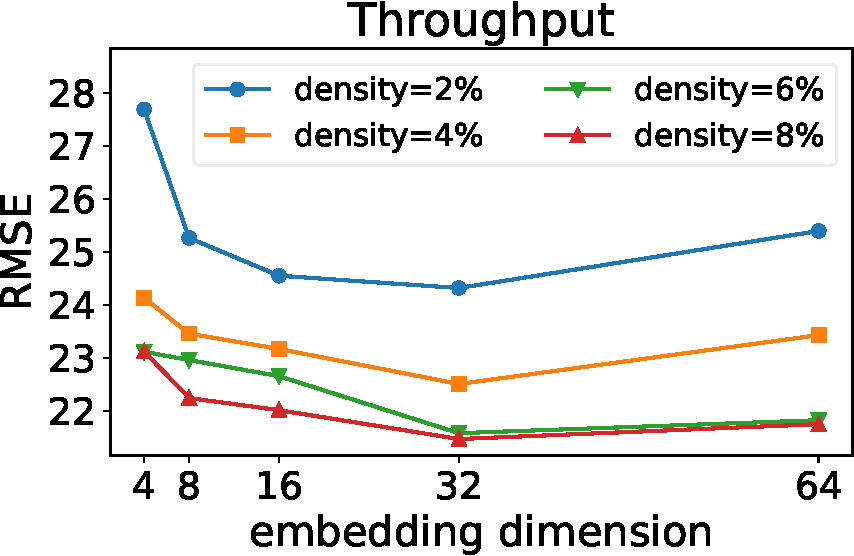
\includegraphics[width=0.7\textwidth]{figs/example.pdf}
    \caption{训练损失下降曲线（截止第50个epoch）}
    \label{fig:interim_loss}
\end{figure}

\section{存在的问题与解决方案}
% 中期检查的关键部分：体现发现问题、分析问题、提出解决思路的过程性。
\subsection{当前遇到的主要困难}
例如：数据质量不足、模型收敛慢、算力限制、模块间接口不兼容等。

\subsection{已尝试的解决措施及效果}
说明尝试了哪些方法（调参、改结构、数据增强等），效果如何（即使无效也值得记录）。

\subsection{后续解决方案}
针对仍未解决的问题，提出下一步的针对性策略（如更换模型、增加数据、简化任务等）。

\section{计划调整与后续工作安排}
% 对照开题报告中的进度表，说明是否需要调整、为什么调整、调整后的新计划。
\subsection{原计划与当前进度对比}
用表格形式列出原计划阶段、原定完成时间、实际完成时间、偏差原因。

\begin{table}[H]
    \centering
    \caption{进度对比表}
    \begin{tabular}{llll}
        \toprule
        阶段任务 & 原计划完成时间 & 实际状态 & 偏差及原因 \\
        \midrule
        数据采集与清洗 & 第3-4周 & 第5周完成 & 数据格式异常，多花1周 \\
        核心模型实现 & 第5-9周 & 第8周完成 & 进展顺利，提前 \\
        系统集成 & 第10-12周 & 进行中 & -- \\
        \bottomrule
    \end{tabular}
\end{table}

\subsection{后续工作计划（调整后）}
\subsubsection{下一阶段重点任务}
列出剩余未完成的主要模块。

\subsubsection{详细时间节点（甘特图或列表）}
例如：
\begin{itemize}
    \item 第11-13周：完成模块C的优化与调参
    \item 第14-15周：系统联调与完整测试
    \item 第16周：撰写结题报告、制作答辩PPT
\end{itemize}


\section{成员分工及进展情况}
% 体现个人在过程中的贡献，便于过程考核。
用表格列出每位成员在中期阶段承担的具体任务、完成比例、工作量评估等。

\begin{table}[H]
    \centering
    \caption{成员分工明细表}
    \begin{tabular}{llll}
        \toprule
        姓名 & 主要任务 & 完成进度 & 存在问题 \\
        \midrule
        成员1 & 模型设计与实验 & 90\% & 调参耗时较长 \\
        成员2 & 数据清洗与前端 & 80\% & 接口对接待完成 \\
        \bottomrule
    \end{tabular}
\end{table}

\section{阶段总结与反思}
% 对整个中期阶段进行回顾，提炼经验教训，展现研究过程的思维成长。
总结截至目前项目的主要收获、不足之处、对后续工作的启发等。可作为中期报告的收尾。

 
\bibliography{ref}
% 参考文献主要包含实验过程中涉及到的参考资料或者借鉴别人的材料等，如无可删除本节。 



\end{document}